\item \points{1b}

Please implement the Disjoint Linear Upper Confidence Bound (LinUCB) algorithm from \href{https://arxiv.org/pdf/1003.0146.pdf}{paper} in ~submission.py~. Below we have provided a snippet of Algorithm 1 from the listed paper. For a thorough description of terms please read through the paper.

\begin{figure}[H]
\centering
  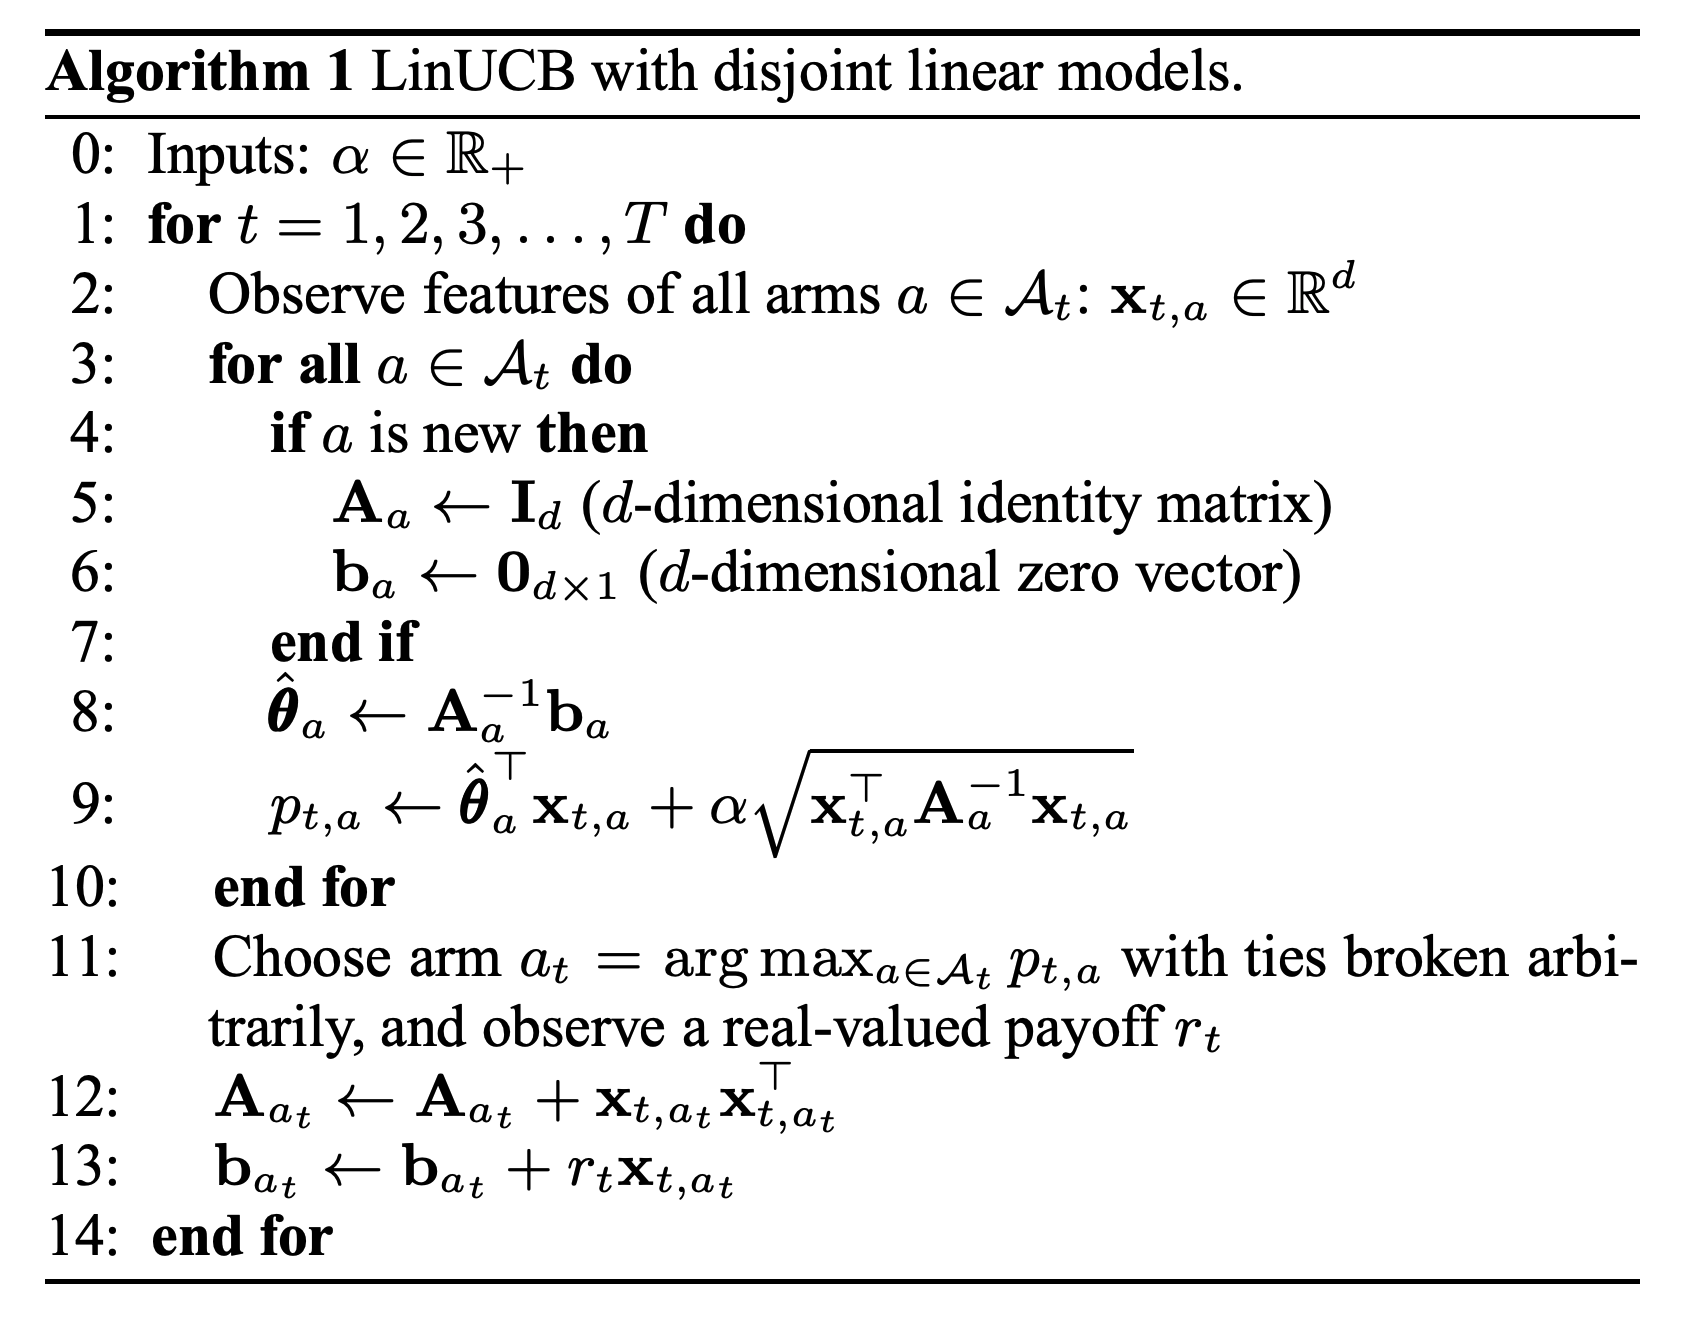
\includegraphics[width=.5\linewidth]{images/linucb_algorithm.png}
  \caption{Definition of the disjoint linear UCB algorithm taken from \href{https://arxiv.org/pdf/1003.0146.pdf}{paper}}
\end{figure}

Run the LinUCB algorithm with the following command:

\begin{lstlisting}
$ python run.py --model linucb
\end{lstlisting}

You should see the total\_fraction\_correct to be above 0.64, though the results may vary per run.

\textit{Note 1: please feel free to adjust the --alpha argument, but you don't have to.}

\textit{Note 2: for arbitrary tie breaking in action selection please simply use ~np.argmax()~.}
